\documentclass[a4paper]{article}
\usepackage[warn]{mathtext}
\usepackage[utf8]{inputenc}
\usepackage[T2A]{fontenc}
\usepackage[english,russian]{babel}
\usepackage{multicol}
\usepackage{fancyhdr}
\usepackage{graphicx}
\usepackage{microtype}
\usepackage{wrapfig}
\usepackage{amsmath}
\usepackage{floatflt}
\usepackage{geometry} \geometry{verbose,a4paper,tmargin=2cm,bmargin=2cm,lmargin=1.5cm,rmargin=1.5cm}
\usepackage{float}
\usepackage{amssymb}
\usepackage{caption}
\usepackage{epsfig}
\usepackage{newunicodechar}

\begin{document}

\graphicspath{ {pictures/} }

\begin{titlepage}
	\centering
	\vspace{5cm}
    {\scshape\LARGE Московский физико-технический институт\par}
	\vspace{5cm}
	{\scshape\Large Лабораторная работа по радиотехнике \par}
	\vspace{1cm}
    {\huge\bfseries  №5 Генераторы синусоидальных колебаний с кварцевой стабилизацией частоты \par}
	\vspace{1cm}
	\vfill
    \begin{flushright}
        {\large выполнил студент Б04-852 группы ФЭФМ}\par
        \vspace{0.3cm}
        {\LARGE Яромир Водзяновский}
    \end{flushright}
	\vfill
Долгопрудный, 2021
% Bottom of the page
\end{titlepage}

\pagestyle{fancy} 
\fancyhead[L]{Радиотехника   }
% \fancyhead[L]{Закон Кюри-Вейса    $( *{^\circ}< >^{\circ}*)$}
\fancyhead[R]{Лабораторная работа}
\fancyhead[C]{}
\fancyfoot[C]{ \noindent\rule{\textwidth}{0.4pt} \thepage }

\newcommand{\ap}{\approx}
\newcommand{\cb}[1]{\begin{center}\fbox{#1} \end{center}}
\newcommand{\cc}[1]{\begin{center} #1 \end{center}}

\newpage



\section{Резонансный усилитель}


\begin{enumerate}
    \item Соберем схему на рис. \ref{scheme_1}. \par

    \begin{figure}[H]
        \begin{center}
            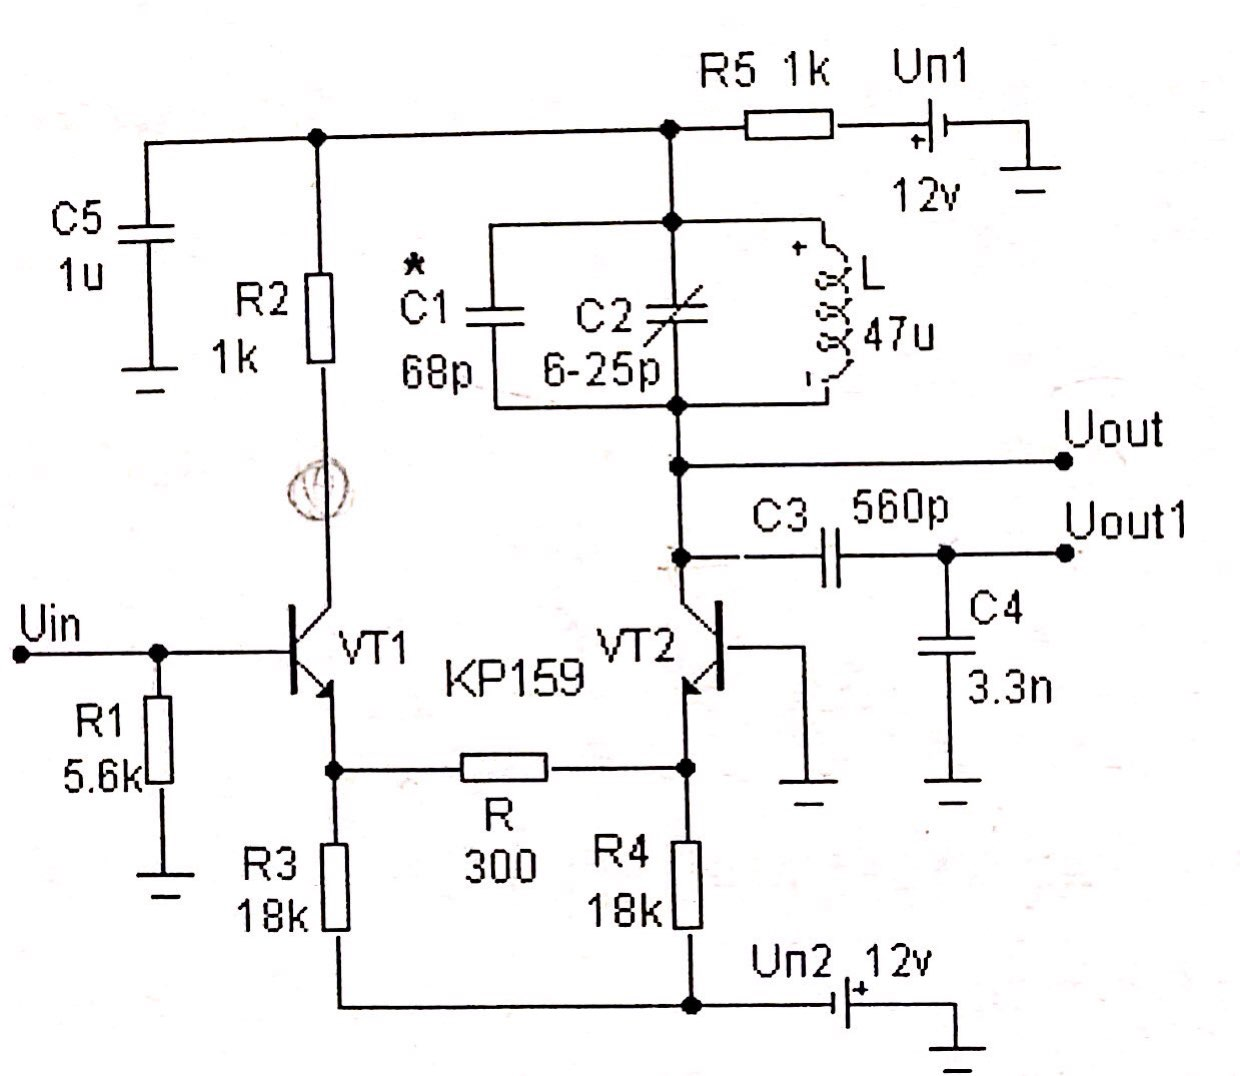
\includegraphics[scale = 0.2]{scheme1.jpg}
            \caption{Схема резонанасного усилителя}
            \label{scheme_1}
        \end{center}
    \end{figure}

    Выход усилителя $U_{out}$, напряжение $U_{out1}$ - выход цепи обратной связи. Они связаны соотношением:
    $$\beta = \frac{U_{out1}}{U_{out}} = \frac{C_3}{C_3 + C_4} \approx \frac{1}{7}$$
    Измерим потенциалы на всех электродах транзисторов. Определим токи эмиттеров $I_{E1}, \; I_{E2}$ и крутизну транзисторов $S = I_C/U_T$.

    \begin{center}
        T1: $U_Б = 0$, $U_k = 8,66 V$, $U_э = -0.52 V$ \par 
        T2: $U_Б = 0$, $U_k = 8,66 V$, $U_э = -0.6 V$
    \end{center}

    \begin{center}
        \fbox{$U_{БЭ_1} = 0.6  \;  V, \;\;\; U_{БЭ_2} = 0.52 \; V$}
    \end{center}

    \begin{center}
        \fbox{$I_{k1} = 50\; mkA$}
        \fbox{$S_1 = \frac{I_{k1}}{U_{БЭ}} \approx 10^{-4}$}
        \fbox{$I_{э1} = 475  \; mkA, \;\;\; I_{э2} = 476 \; mkA$}
    \end{center}



    \item Подадим входной сигнал $U_{in}$ от генератора. Изменяя частоту сигнала налюдаем переменное напряжение на выходе. Найдем резонанс. \par
    \begin{center}
        \fbox{$f_p = 1.1\; MGz$}
    \end{center} 

    \item На резонансной частоте $f_p$ снимем АЧХ усилителя изменяя амплитуду $U_{m_{in}}$ от 10 до 500 мВ, занесем результат в таблицу \ref{t1}. Построим график зависимости 
    $K = U_{m_{out}}/ U_{m_{in}}$ от амплитуды входного сигнала рис. \ref{gr1}.

    \begin{table}[H]
        \centering
        \begin{center}
        \end{center}
        \vspace{0.1cm}
        \begin{tabular}{|c|c|c|c|c|c|c|c|c|}
            \hline
            $U_{out}$, mV  & 150  & 300&450 & 745& 1460& 2700&3388 & 3700  \\ 
            \hline
            $U_{in}$, mV   & 10 &  20 &  30 &50& 100&200 & 300 &  500  \\
            \hline
            \end{tabular}
            \caption{Зависимость $U_{out}$  от $U_{in}$}
            \label{t1}
    \end{table}

    \begin{figure}[H]
        \begin{center}
            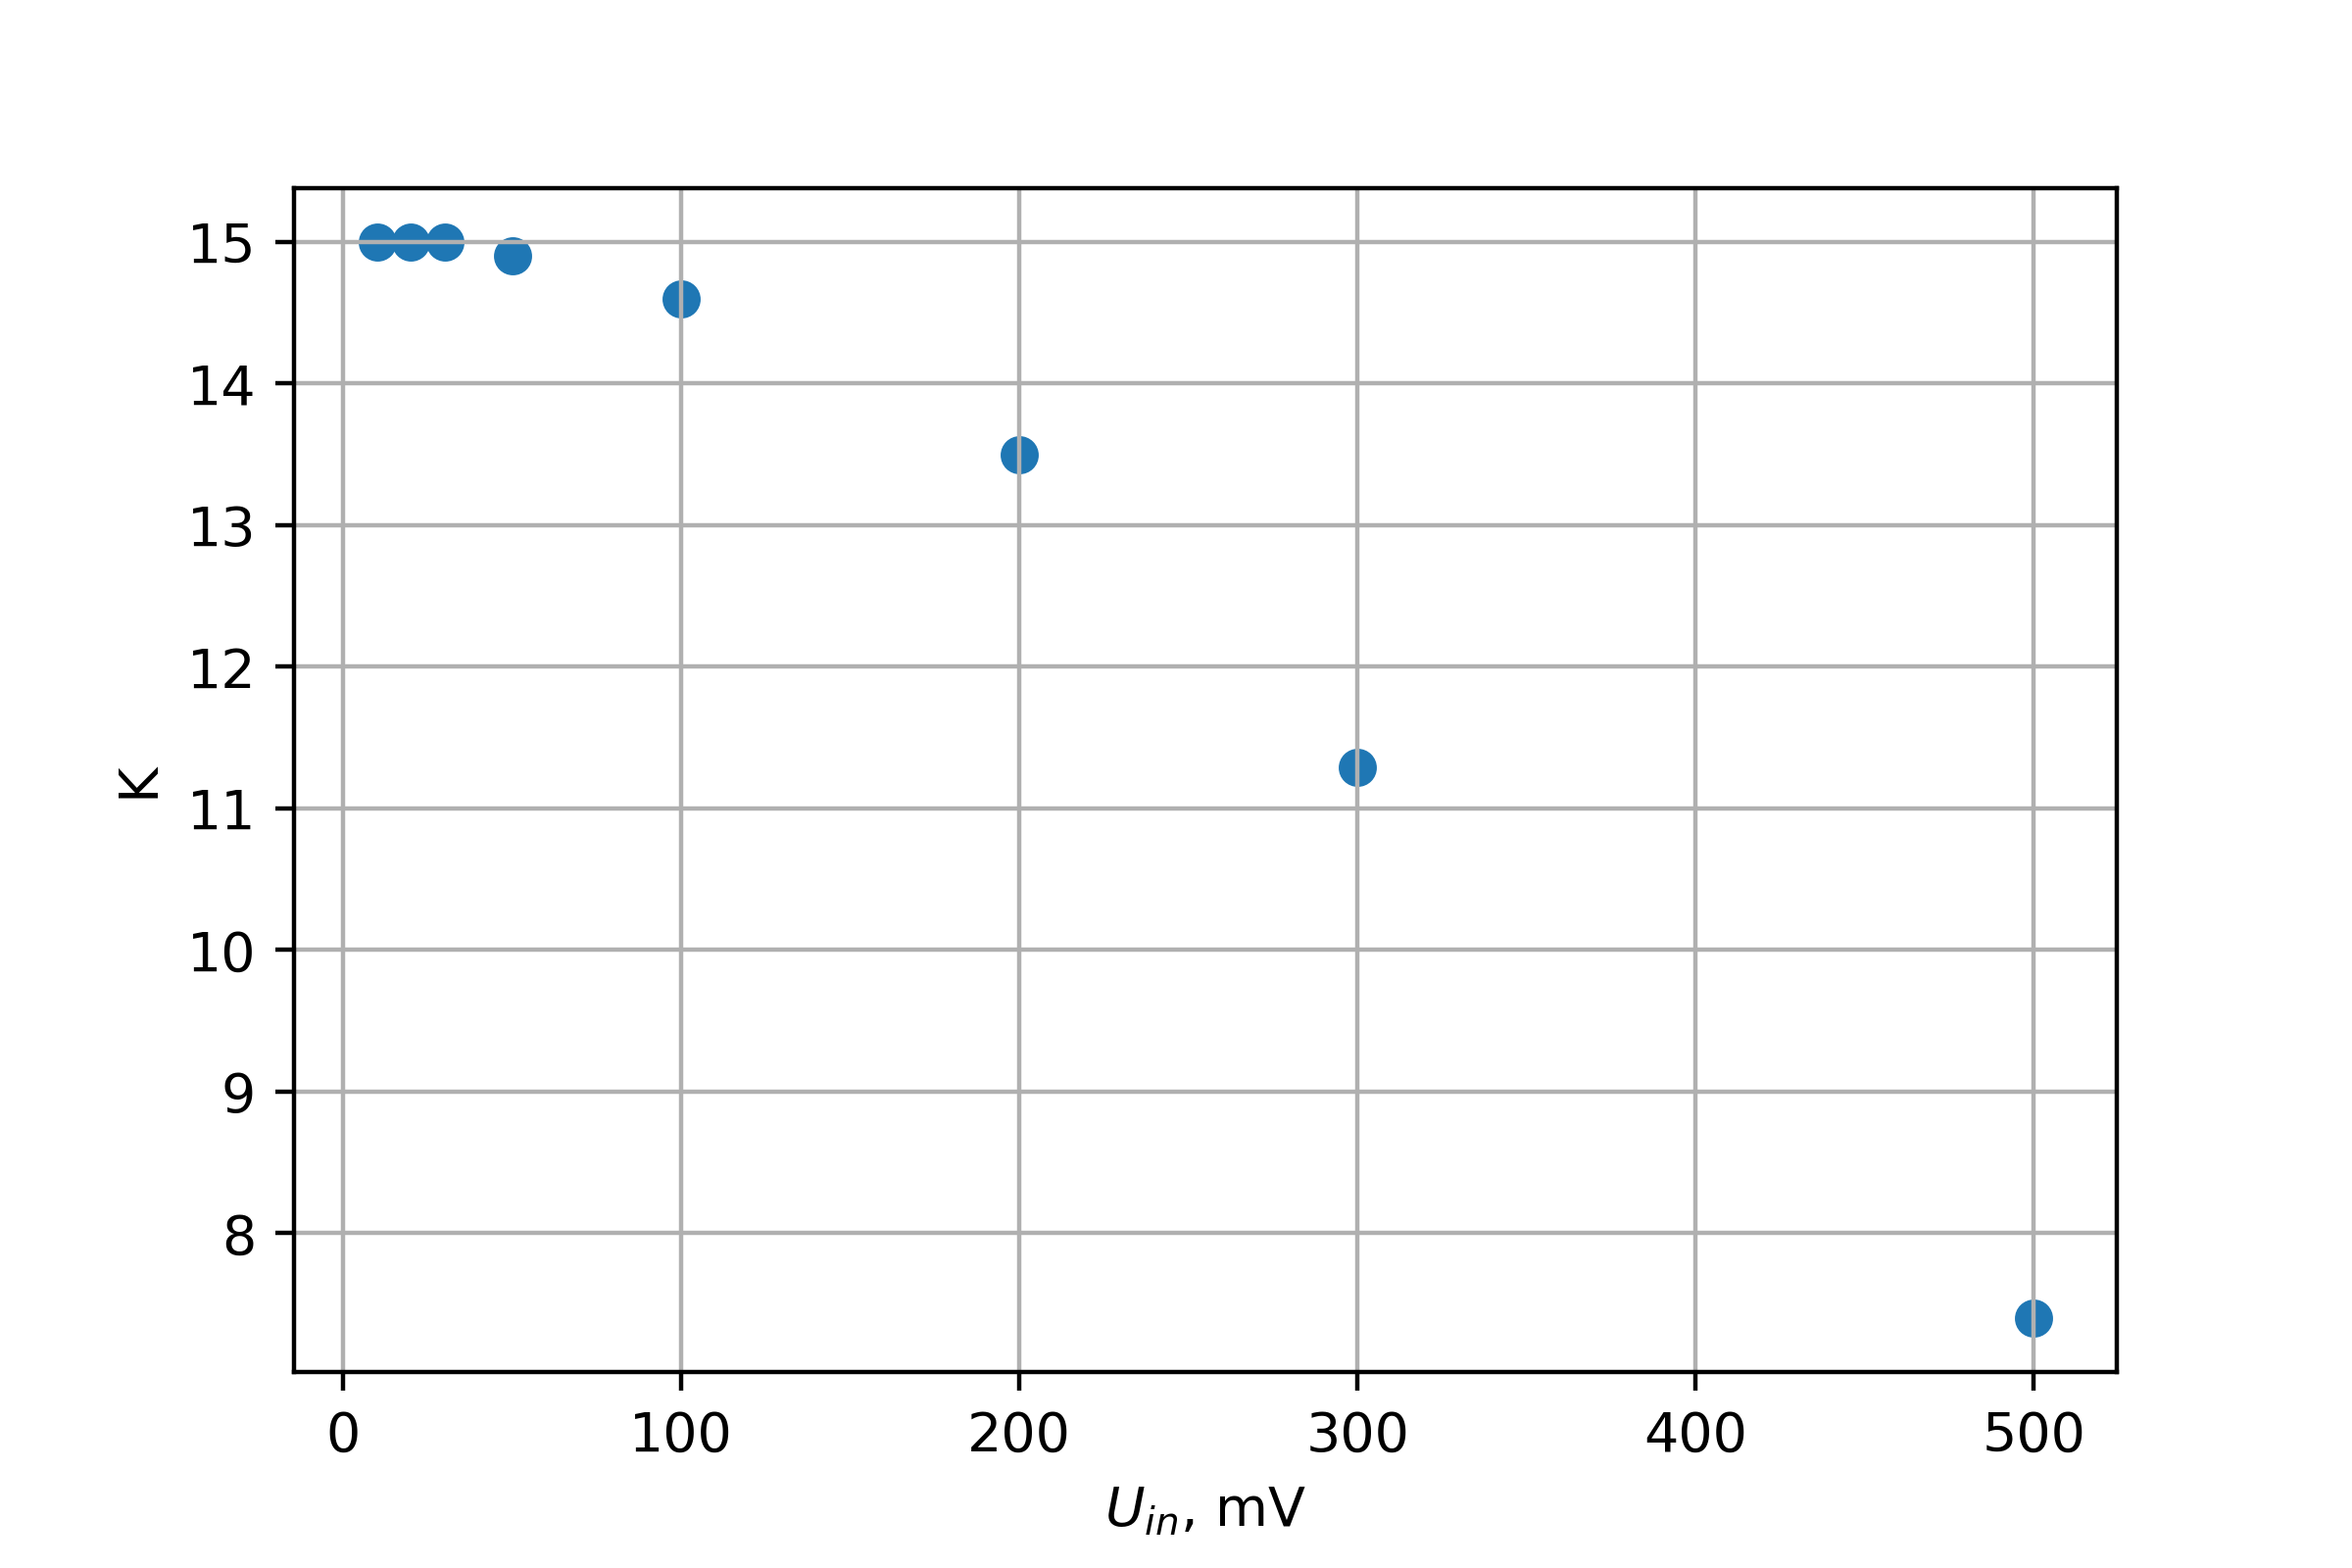
\includegraphics[scale = 1]{gr1.png}
            \caption{Зависимость $K(U_{in})$}
            \label{gr1}
        \end{center}
    \end{figure}


    \item Измерим резонансный коэффициент усиления для случая $R=0$, соединив накоротко эмиттеры у транзисторов. \par 
    $U_{in} = 0.01 \;V \;\;\; U_{out} = 0,45\; V$
    \begin{center}
        \fbox{$K \approx 45$}
    \end{center}


    \item Снимем зависимость коэффициента усиления от частоты входного сигнала при амплитуде $U_{m_{in}} = 20\; mV$, соответсвующей линейному участку АЧХ и занесем в таблицу \ref{t2}. Построим эту зависимость рис. \ref{gr2}.
    Определим полосу пропускания $\Delta f_{0.7}$ и добротность $Q = f_{p}/\Delta f_{0.7}$. \par 

    \begin{center}
        \fbox{$f_н = 1050\;kGz, \;\;\; f_в = 1100 \; kGz$}
    \end{center}

    \begin{center}
        \fbox{$Q \approx 22$}
        \fbox{$K_{max} \approx 14.45$}
    \end{center}

    \begin{table}[H]
        \centering
        \begin{center}
        \end{center}
        \vspace{0.1cm}
        \begin{tabular}{|c|c|c|c|c|c|c|c|c|c|c|}
            \hline
            $f$, kGz  &400& 500& 700& 900& 1000& 1050& 1070& 1100& 1120& 1150  \\ 
            \hline
            $U_{out}$, mV &7.2& 9.45& 17& 40& 94& 224& 289& 210& 137& 97.5  \\
            \hline
            \end{tabular}
            \caption{Зависимость $U_{out}$  от $f$}
            \label{t2}
    \end{table}

    
    \begin{figure}[H]
        \begin{center}
            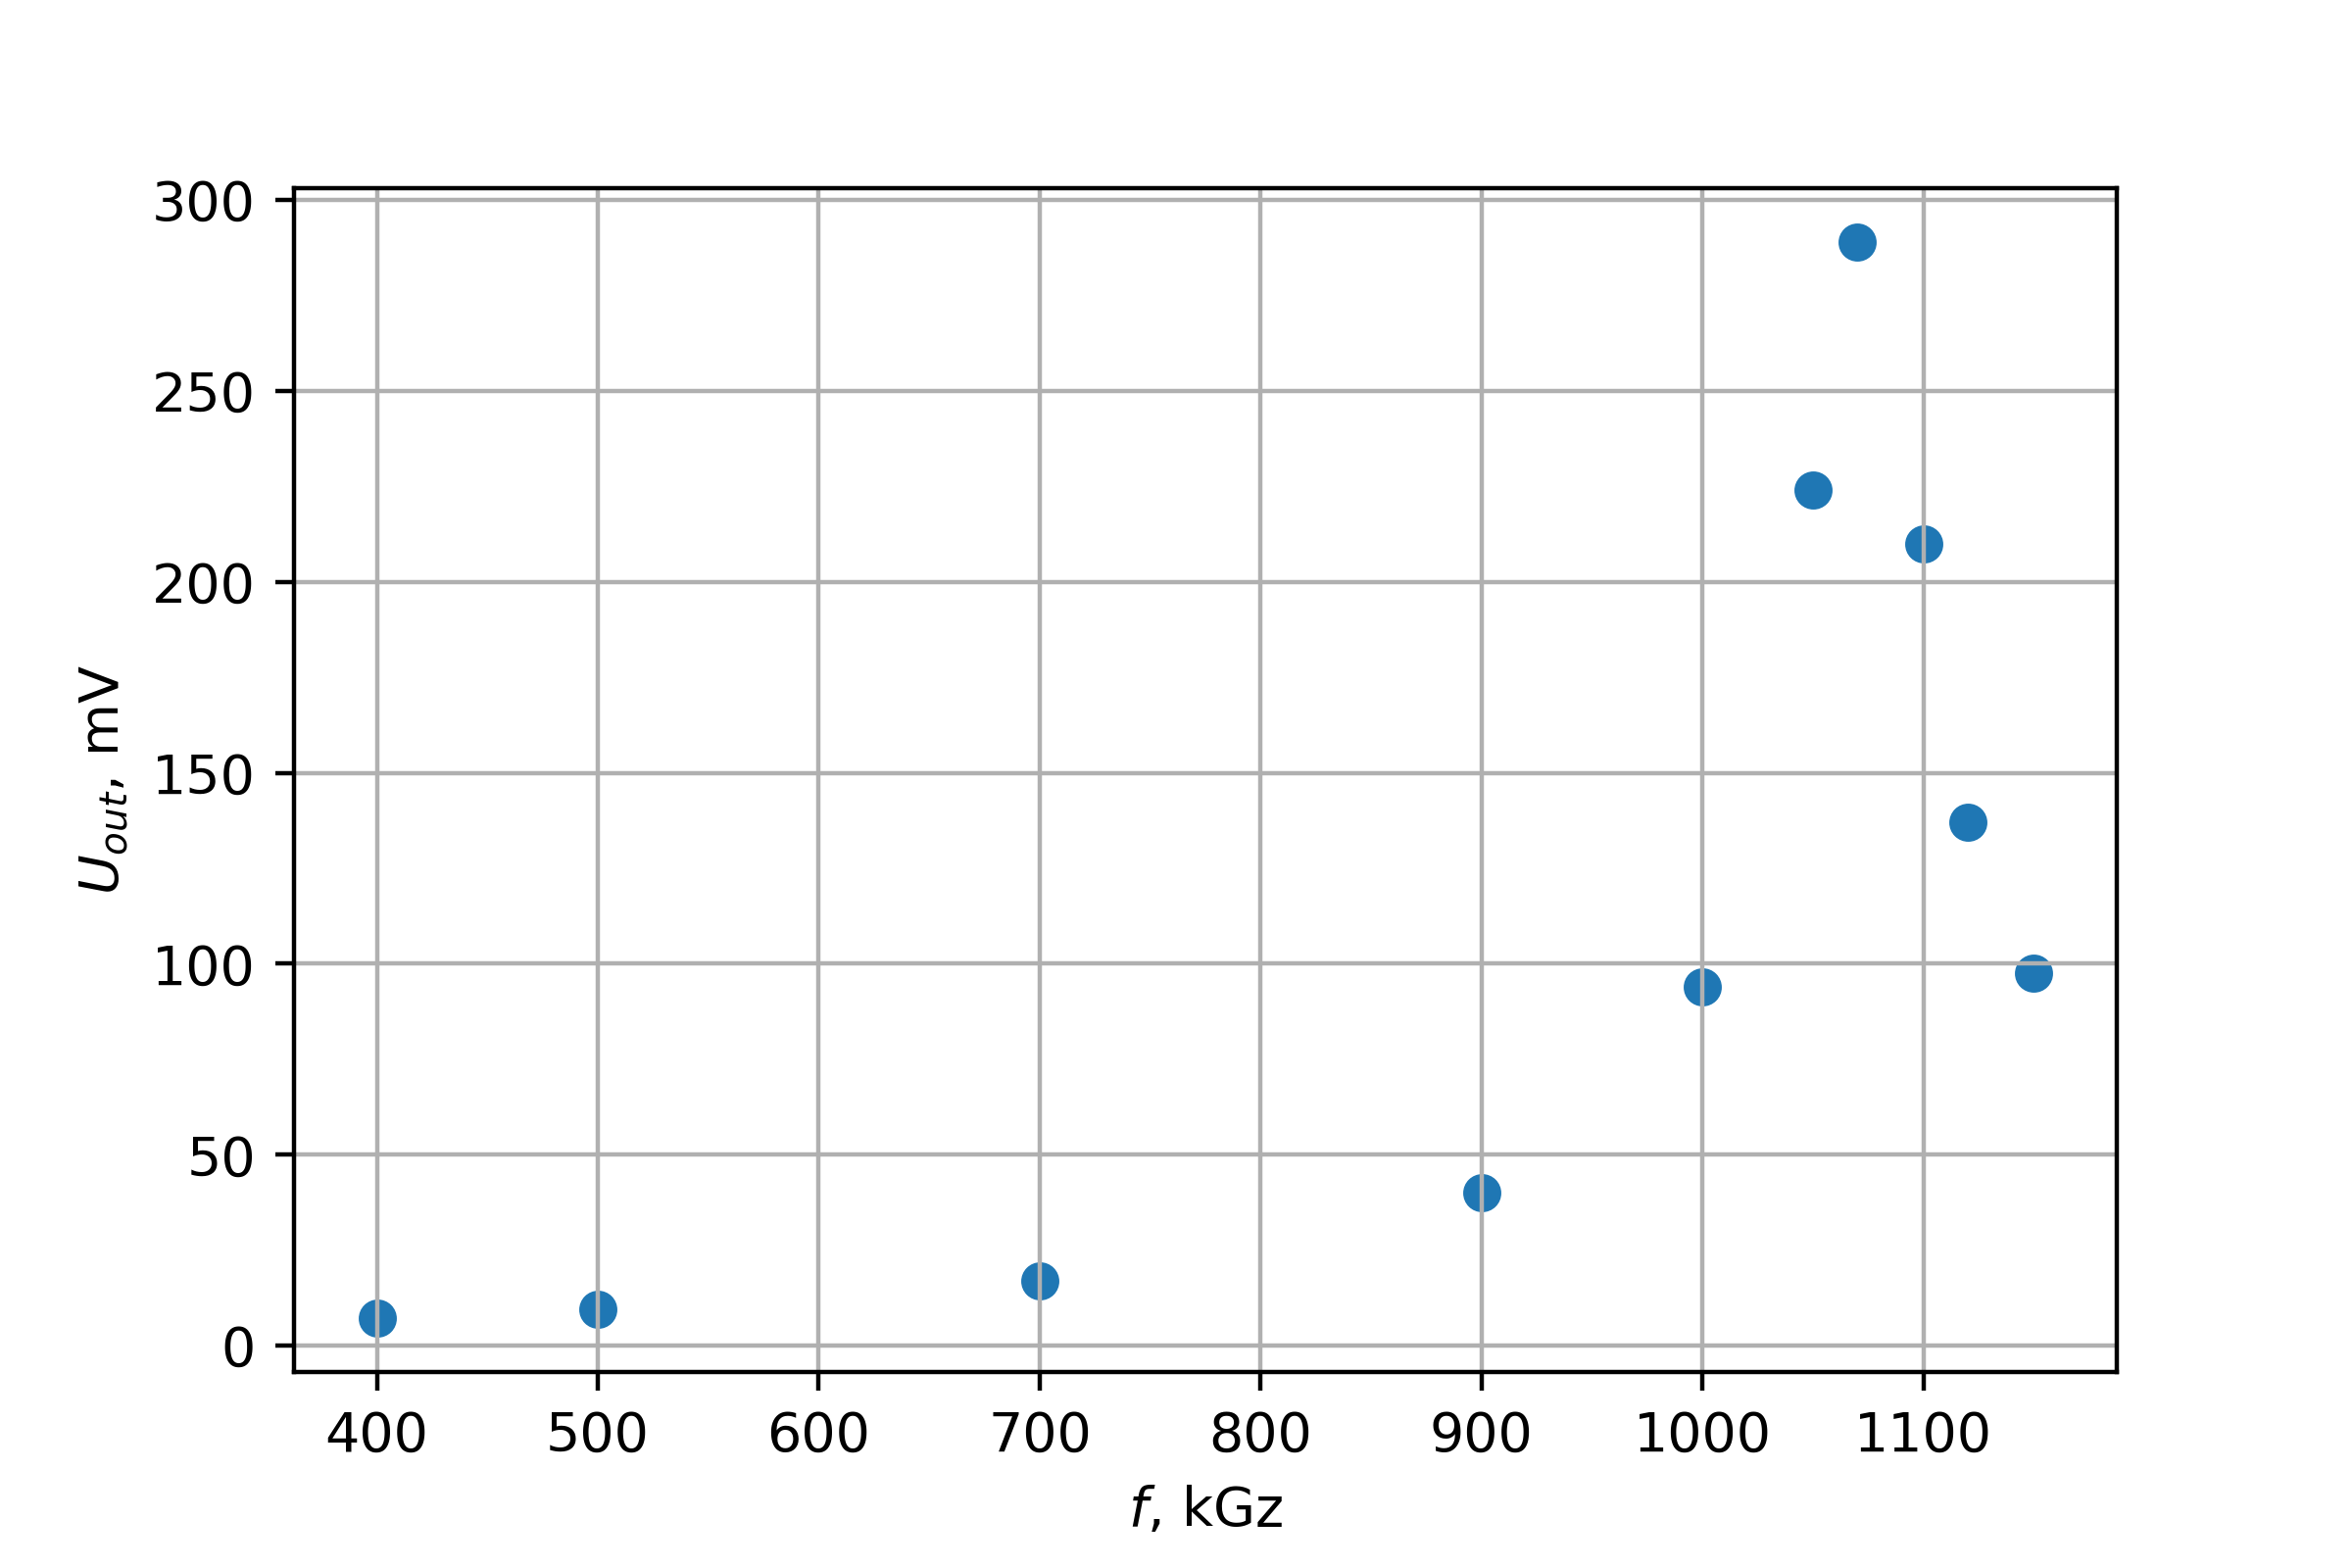
\includegraphics[scale = 1]{gr2.png}
            \caption{Зависимость $K(f)$}
            \label{gr2}
        \end{center}
    \end{figure}

\end{enumerate}



\section{Кварцевый генератор с использованием последовательного резонанса кварца}


\begin{enumerate}
    \item Замкнем цепь обратной связи как на рис. \ref{scheme_2}. Вместо кварца подключим резистор $R = 300\; \Omega.$ Измерим частоту выходнго колебания. \par 
    \begin{center}
        \fbox{$f \approx 1\; MGz$}
    \end{center}
    
    \begin{figure}[H]
        \begin{center}
            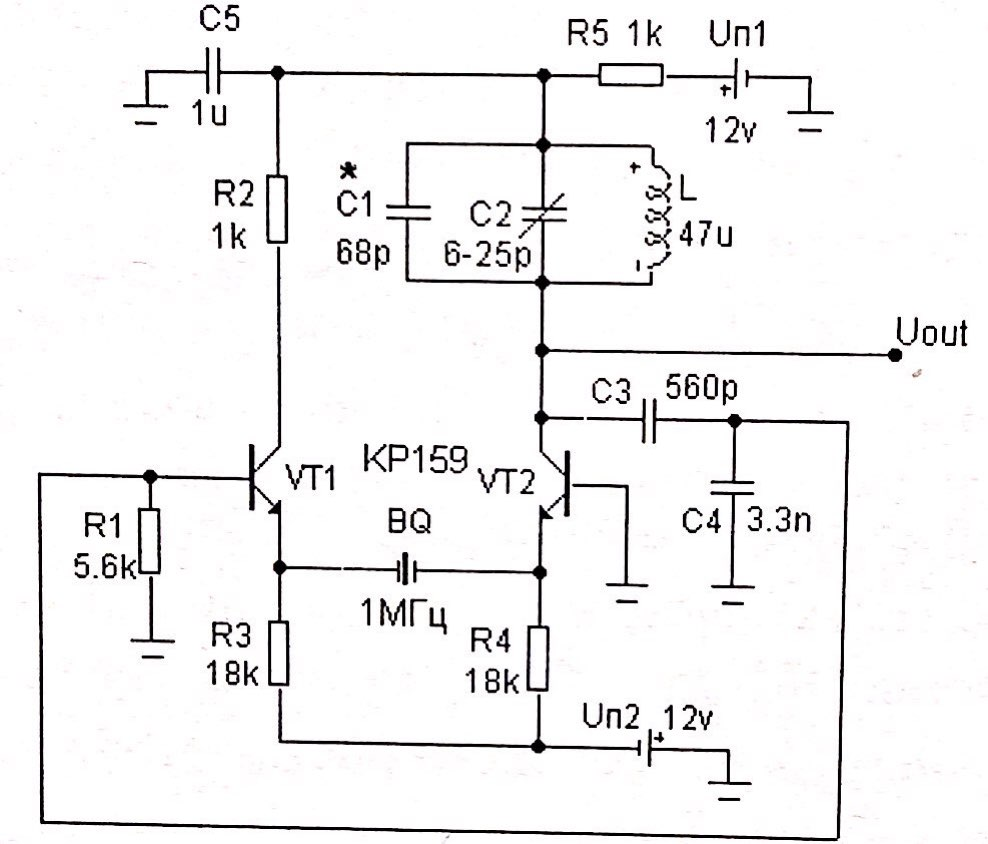
\includegraphics[scale = 0.2]{scheme_2.jpg}
            \caption{Схема кварцевого генератора с использованием последовательного резонанса кварца}
            \label{scheme_2}
        \end{center}
    \end{figure}


    \item Включим между эмиттерами кварцевый резонатор вместо $R$. Измерим частоту колебаний. \par 
    
    Чтобы возникли колебания пришлось увеличить емкость $C_1 = 100 \div 120\; pF$.
    \begin{center}
        \fbox{$f \approx 1\; MGz$}
    \end{center}


    \item Измерим добротность кварцевого резонатора. \par 
    Расстроим LC-контур, внесем $\Delta C = 13 \div 16\; pF$

    \begin{center}
        Без кварца: $\Delta f \approx 9\; Gz$ \par 
        С кварцем: $\Delta f_k \approx 26\; kGz$
    \end{center}

    \begin{center}
        \fbox{$Q_k = \Delta f_k/\Delta f \cdot Q \approx 63555$}
    \end{center}



    \item Восстановим настройку контура в резонанс.  \par 
    
    Определим электрические параметры кварцевого резонатора. Включим последователно с кварцем конденсатор $C_s = 130 \div 160\; pF$, измерим изменение $\Delta f_k$.

    \begin{center}
        \fbox{$C_k = 2 C_s \frac{\Delta f_k}{f_k} = 7.28 \cdot 10^{-3}\; pF$} \par 
        \fbox{$L_k = \frac{1}{4 \pi^2 f_k^2 C_k} = 3.47\; Гн$} \par 
        \fbox{$\rho_k = \sqrt{L_k/C_k} = 21.8\; M\Omega$} \par 
        \fbox{$r_k = \frac{\rho_k}{Q_k} = 338.3\; \Omega$}
    \end{center}

    \item Исследуем стабильность частоты кварцевого генератора при изменении питающего напряжения $U_{п2}$ от 8 до 12 В. Результаты внесем в таблицу \ref{t3} без кварца и с кварцем.
    
    \begin{table}[H]
        \centering
        \begin{center}
        \end{center}
        \vspace{0.1cm}
        \begin{tabular}{|c|c|c|c|c|c|}
            \hline
            $U_{п2}$, V & 8&9&10&11&12 \\ 
            \hline
            $f$, kGz без кварца  &997.243&  996.745& 996.163& 995.854& 995.264 \\ 
            \hline
            $f$, MGz с кварцем  &1.000016&  1.000017& 1.000018& 1.000017& 1.000018 \\ 
            \hline
            \end{tabular}
            \caption{Стабильность частоты}
            \label{t3}
    \end{table}


\end{enumerate}



\section{Кварцевый генератор с использованием кварца в качестве индуктивности}

\begin{enumerate}
    \item Соберем схему рис. \ref{scheme_3}
    
    Измерим частоту колебаний генератора, рподстроив в резонанс LC-контур. 
    \begin{center}
        \fbox{$f \approx 980\; kGz$}
    \end{center}

    \begin{figure}[H]
        \begin{center}
            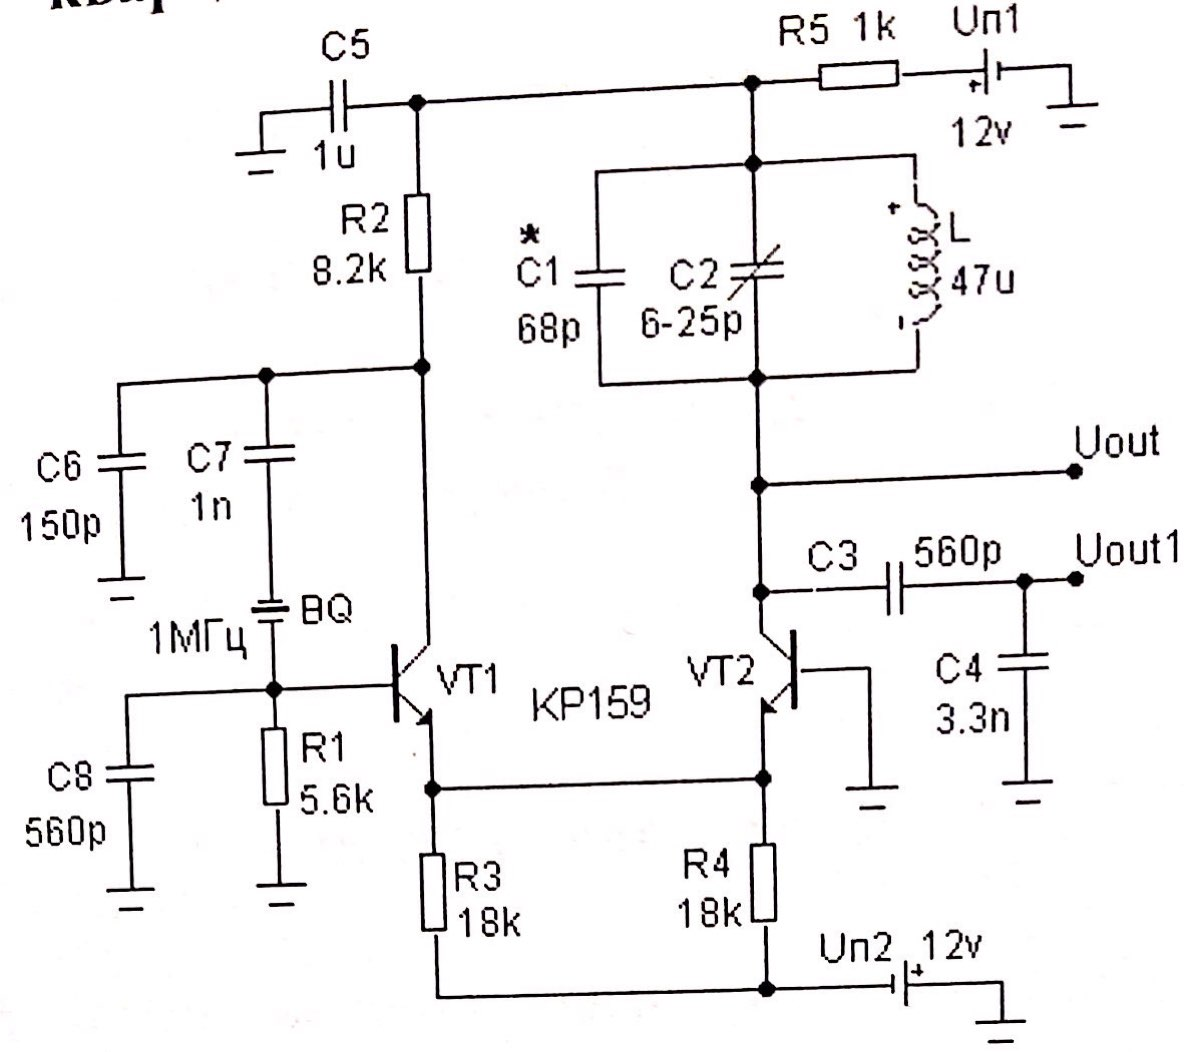
\includegraphics[scale = 0.2]{scheme_3.jpg}
            \caption{Схема кварцевого генератора с использованием кварца в качестве индуктивности}
            \label{scheme_3}
        \end{center}
    \end{figure}

    \item Измерим ход частоты колебаний генератора при изменении емкости конденсатора $C_7$, подключив парралельно $430 \div 510\; pF$.
    \begin{center}
        \fbox{$f = 980.453\; kGz$}
    \end{center}
    \item Исследуем стабильность частоты кварцевого генератора при изменении питающего напряжения $U_{п2}$. Снимем зависимость частоты генератора от значений напряжения 
    $U_{п2}$ от 8 до 12 В. Результат в таблице \ref{t5}.

    \begin{table}[H]
        \centering
        \begin{center}
        \end{center}
        \vspace{0.1cm}
        \begin{tabular}{|c|c|c|c|c|c|}
            \hline
            $U_{п2}$, V & 8&9&10&11&12 \\ 
            \hline
            $f$, MGz  &1.000016&  1.000017& 1.000018& 1.000017& 1.000018 \\ 
            \hline
            \end{tabular}
            \caption{Стабильность частоты генератора}
            \label{t5}
    \end{table}


\end{enumerate}

\end{document}